    \section{Ogólna struktura projektu}
    \subsection{Wprowadzenie}
Zadaniem jest skonstruowanie wzmacniacza biopotencjałów. 
Jego struktura będzie się składać z: stopnia wejściowego opartego na
wzmacniaczu pomiarowym [model], wstępnym filtrze pasmowo przepustowym, 
bardziej selektywnym filtrze pasmowo przepustowym
oraz filtrze typu Notch eliminującym zakłócenia sieciowe 50 Hz.
\subsection{Ogólna struktura wzmacniacza}
Poniżej przedstawiono ogólną strukturę wzmacniacza biopotencjałów. 
Wyróżnione zostały opisane
\begin{figure}[H]
\centering
\setlength{\fboxrule}{2pt}
\setlength{\fboxsep}{0pt}
\fbox{
    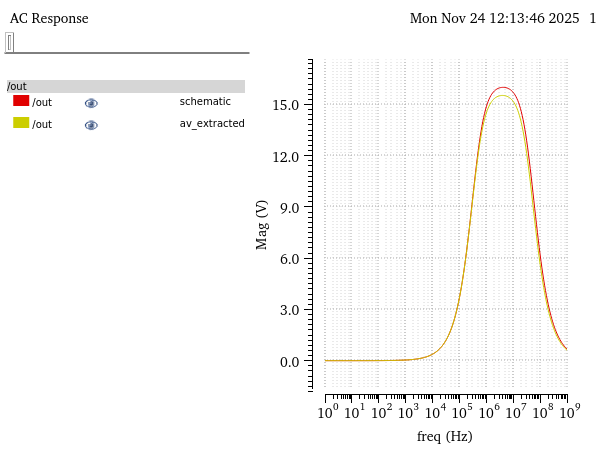
\includegraphics[width=0.4\textwidth]{figures/example.png}
}
\caption{Uproszczony schemat projektowanego toru pomiarowego.}
\end{figure}